

\documentclass[11pt,compress,t,notes=noshow, xcolor=table]{beamer}
\usepackage[]{graphicx}\usepackage[]{color}
% maxwidth is the original width if it is less than linewidth
% otherwise use linewidth (to make sure the graphics do not exceed the margin)
\makeatletter
\def\maxwidth{ %
  \ifdim\Gin@nat@width>\linewidth
    \linewidth
  \else
    \Gin@nat@width
  \fi
}
\makeatother

\definecolor{fgcolor}{rgb}{0.345, 0.345, 0.345}
\newcommand{\hlnum}[1]{\textcolor[rgb]{0.686,0.059,0.569}{#1}}%
\newcommand{\hlstr}[1]{\textcolor[rgb]{0.192,0.494,0.8}{#1}}%
\newcommand{\hlcom}[1]{\textcolor[rgb]{0.678,0.584,0.686}{\textit{#1}}}%
\newcommand{\hlopt}[1]{\textcolor[rgb]{0,0,0}{#1}}%
\newcommand{\hlstd}[1]{\textcolor[rgb]{0.345,0.345,0.345}{#1}}%
\newcommand{\hlkwa}[1]{\textcolor[rgb]{0.161,0.373,0.58}{\textbf{#1}}}%
\newcommand{\hlkwb}[1]{\textcolor[rgb]{0.69,0.353,0.396}{#1}}%
\newcommand{\hlkwc}[1]{\textcolor[rgb]{0.333,0.667,0.333}{#1}}%
\newcommand{\hlkwd}[1]{\textcolor[rgb]{0.737,0.353,0.396}{\textbf{#1}}}%
\let\hlipl\hlkwb

\usepackage{framed}
\makeatletter
\newenvironment{kframe}{%
 \def\at@end@of@kframe{}%
 \ifinner\ifhmode%
  \def\at@end@of@kframe{\end{minipage}}%
  \begin{minipage}{\columnwidth}%
 \fi\fi%
 \def\FrameCommand##1{\hskip\@totalleftmargin \hskip-\fboxsep
 \colorbox{shadecolor}{##1}\hskip-\fboxsep
     % There is no \\@totalrightmargin, so:
     \hskip-\linewidth \hskip-\@totalleftmargin \hskip\columnwidth}%
 \MakeFramed {\advance\hsize-\width
   \@totalleftmargin\z@ \linewidth\hsize
   \@setminipage}}%
 {\par\unskip\endMakeFramed%
 \at@end@of@kframe}
\makeatother

\definecolor{shadecolor}{rgb}{.97, .97, .97}
\definecolor{messagecolor}{rgb}{0, 0, 0}
\definecolor{warningcolor}{rgb}{1, 0, 1}
\definecolor{errorcolor}{rgb}{1, 0, 0}
\newenvironment{knitrout}{}{} % an empty environment to be redefined in TeX

\usepackage{alltt}
\newcommand{\SweaveOpts}[1]{}  % do not interfere with LaTeX
\newcommand{\SweaveInput}[1]{} % because they are not real TeX commands
\newcommand{\Sexpr}[1]{}       % will only be parsed by R
\newcommand{\xmark}{\ding{55}}%


\usepackage[english]{babel}
\usepackage[utf8]{inputenc}

\usepackage{dsfont}
\usepackage{verbatim}
\usepackage{amsmath}
\usepackage{amsfonts}
\usepackage{amssymb}
\usepackage{bm}
\usepackage{csquotes}
\usepackage{multirow}
\usepackage{longtable}
\usepackage{booktabs}
\usepackage{enumerate}
\usepackage[absolute,overlay]{textpos}
\usepackage{psfrag}
\usepackage{algorithm}
\usepackage{algpseudocode}
\usepackage{eqnarray}
\usepackage{arydshln}
\usepackage{tabularx}
\usepackage{placeins}
\usepackage{tikz}
\usepackage{setspace}
\usepackage{colortbl}
\usepackage{mathtools}
\usepackage{wrapfig}
\usepackage{bm}
\usepackage{amsmath}
\usepackage{pifont}
\usepackage{xcolor} %colored math symbols

\usetikzlibrary{shapes,arrows,automata,positioning,calc,chains,trees, shadows}
\tikzset{
  %Define standard arrow tip
  >=stealth',
  %Define style for boxes
  punkt/.style={
    rectangle,
    rounded corners,
    draw=black, very thick,
    text width=6.5em,
    minimum height=2em,
    text centered},
  % Define arrow style
  pil/.style={
    ->,
    thick,
    shorten <=2pt,
    shorten >=2pt,}
}

\usepackage{subfig}

% Defines macros and environments
\usepackage{../../style/lmu-lecture}


\let\code=\texttt
\let\proglang=\textsf

\setkeys{Gin}{width=0.9\textwidth}

\setbeamertemplate{frametitle}{\expandafter\uppercase\expandafter\insertframetitle}

\usepackage{bbm}
% basic latex stuff
\newcommand{\pkg}[1]{{\fontseries{b}\selectfont #1}} %fontstyle for R packages
\newcommand{\lz}{\vspace{0.5cm}} %vertical space
\newcommand{\dlz}{\vspace{1cm}} %double vertical space
\newcommand{\oneliner}[1] % Oneliner for important statements
{\begin{block}{}\begin{center}\begin{Large}#1\end{Large}\end{center}\end{block}}


%new environments
\newenvironment{vbframe}  %frame with breaks and verbatim
{
 \begin{frame}[containsverbatim,allowframebreaks]
}
{
\end{frame}
}

\newenvironment{vframe}  %frame with verbatim without breaks (to avoid numbering one slided frames)
{
 \begin{frame}[containsverbatim]
}
{
\end{frame}
}

\newenvironment{blocki}[1]   % itemize block
{
 \begin{block}{#1}\begin{itemize}
}
{
\end{itemize}\end{block}
}

\newenvironment{fragileframe}[2]{  %fragile frame with framebreaks
\begin{frame}[allowframebreaks, fragile, environment = fragileframe]
\frametitle{#1}
#2}
{\end{frame}}


\newcommand{\myframe}[2]{  %short for frame with framebreaks
\begin{frame}[allowframebreaks]
\frametitle{#1}
#2
\end{frame}}

\newcommand{\remark}[1]{
  \textbf{Remark:} #1
}


\newenvironment{deleteframe}
{
\begingroup
\usebackgroundtemplate{
\includegraphics[width=\paperwidth,height=\paperheight]{../style/color/red.png}}
 \begin{frame}
}
{
\end{frame}
\endgroup
}
\newenvironment{simplifyframe}
{
\begingroup
\usebackgroundtemplate{
\includegraphics[width=\paperwidth,height=\paperheight]{../style/color/yellow.png}}
 \begin{frame}
}
{
\end{frame}
\endgroup
}\newenvironment{draftframe}
{
\begingroup
\usebackgroundtemplate{
\includegraphics[width=\paperwidth,height=\paperheight]{../style/color/green.jpg}}
 \begin{frame}
}
{
\end{frame}
\endgroup
}
% https://tex.stackexchange.com/a/261480: textcolor that works in mathmode
\makeatletter
\renewcommand*{\@textcolor}[3]{%
  \protect\leavevmode
  \begingroup
    \color#1{#2}#3%
  \endgroup
}
\makeatother


\input{../../latex-math/basic-math}
\input{../../latex-math/basic-ml}
\input{../../latex-math/ml-nn}

\newcommand{\titlefigure}{figure/rnn_sample_z5.png}
%modify picture
\newcommand{\learninggoals}{
  \item Why do we need them?
  \item How do they work?
  \item Computational Graph o Recurrent Networks
}

\title{Deep Learning}
\date{}



\begin{document}

\lecturechapter{Recurrent Neural Networks - Introduction}
\lecture{I2DL}

%%%%%%%%%%%%%%%%%%%%%%%%%%%%%%%%%%%%%%%%%%%%%%%%%%%%%%%%%%%%%%%%%%
%%%%%%%%%%%%%%%%%%%%%%%%%%%%%%%%%%%%%%%%%%%%%%%%%%%%%%%%%%%%%%%%%%

\section{Motivation}

\begin{frame} {Motivation for Recurrent Networks}
  \begin{itemize}
    \item The two types of neural network architectures that we've seen so far are fully-connected networks and CNNs.
    \item Their input layers have a fixed size and (typically) only handle fixed-length inputs.
    \item The primary reason: if we vary the size of the input layer, we would also have to vary the number of learnable weights in the network.
    \item This in particular relates to \textbf{sequence data} such as time-series, audio and text.
    \item \textbf{Recurrent Neural Networks (RNNs)} is a class of architectures that allows varying input lengths and properly accounts for the ordering in sequence data.
  \end{itemize}
\end{frame}


%%%%%%%%%%%%%%%%%%%%%%%%%%%%%%%%%%%%%%%%%%%%%%%%%%%%%%%%%%%%%%%%%%

% \frame{
 
% \frametitle{RNNs - What for?}
%   So far we encountered two types of data: tabular data and image data.
%   Suppose we would like to process sequential inputs, such as
%   \begin{itemize}
%     \item Text data (for text recognition, machine translation, sentiment classification)
%     \item Audio signal analysis (music generation, speech recognition)
%     \item Time series analysis (to predict the stock market,DNA sequence analysis).
%   \end{itemize}
%   Can we do that with a convnet?
%   \begin{itemize}
%     \item[]
%   \end{itemize}
%   \begin{centering}
%   \begin{minipage}{0.42\textwidth}
%     \begin{figure}
%         \only<1-2>{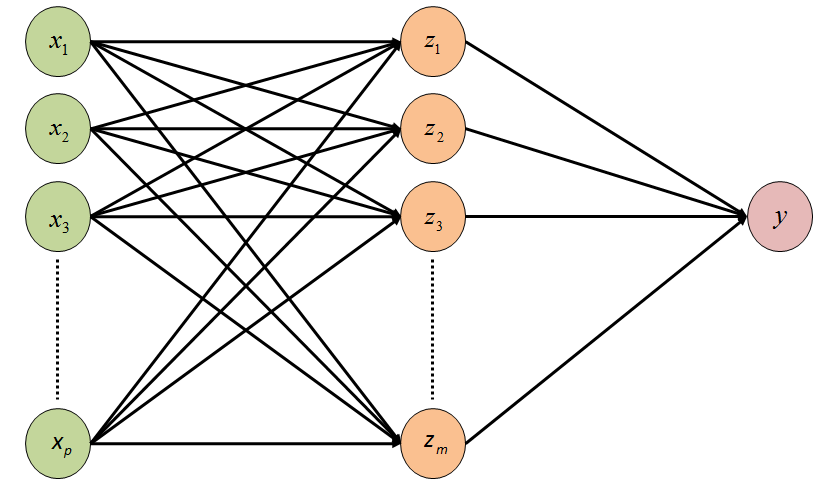
\includegraphics[width=4.5cm]{plots/neuralnet2.png}}
%         \caption{A dense architecture. \textcolor{white}{bla bla bla blabla blabla blabla blabla blabla bla}}
%     \end{figure}
%   \end{minipage}\hfill
%   \begin{minipage}{0.57\textwidth}
%   \vspace{-0.2cm}
%     \begin{itemize}
%       \only<1>{\item[] \textcolor{white}{bla}} % stupid trick to get rid of compiling error
%       \only<2>{\item[] Hardly, the major drawbacks of these models are:} %The major drawbacks of these models for sequential data are:}
%       \only<2>{\begin{itemize}
%         \only<2>{\item \textbf{a fixed input length}. \\ The length of sequential inputs can vary!}
%         \only<2>{\item \textbf{all the examples are independently and identically distributed}. \\ For sequential inputs, there are short and long term temporal dependencies!}
%       \end{itemize}} 
%     \end{itemize}  
%   \end{minipage}
%   \end{centering}
% }
%%%%%%%%%%%%%%%%%%%%%%%%%%%%%%%%%%%%%%%%%%%%%%%%%%%%%%%%%%%%%%%%%%

%\section{RNNs -- The basic idea}

\begin{frame} {RNNs - Introduction}
  \begin{itemize}
    \item \small{Suppose we have some text data and our task is to analyse the \textit{sentiment} in the text.
    \item For example, given an input sentence, such as "This is good news.", the network has to classify it as either 'positive' or 'negative'.
    \item We would like to train a simple neural network (such as the one below) to perform the task.}
  \end{itemize}
  \begin{figure}
      \centering
      \scalebox{0.6}{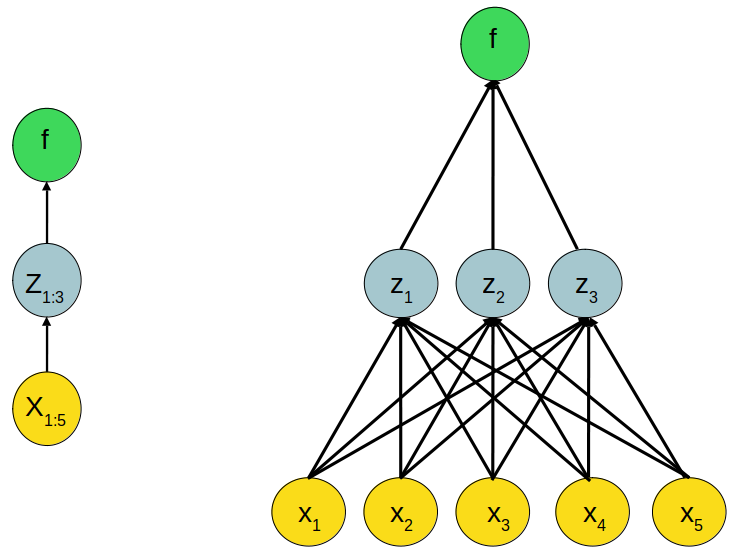
\includegraphics{figure/ffwd.png}}
      \caption{\footnotesize{Two equivalent visualizations of a dense net with a single hidden layer, where the left is more abstract showing the network on a layer point-of-view.}}
  \end{figure}
\end{frame}

\begin{frame} {RNNs - Introduction}
  \begin{itemize}
    \item Because sentences can be of varying lengths, we need to modify the dense net architecture to handle such a scenario.
    \item One approach is to draw inspiration from the way a human reads a sentence; that is, one word at a time.
    \item An important cognitive mechanism that makes this possible is "\textbf{short-term memory}".
    \item As we read a sentence from beginning to end, we retain some information about the words that we have already read and use this information to understand the meaning of the entire sentence.
    \item Therefore, in order to feed the words in a sentence sequentially to a neural network, we need to give it the ability to retain some information about past inputs.
    %\item \texbf{We need to track long-term dependencies.}
  \end{itemize}
\end{frame}
 
\begin{frame} {RNNs - Introduction}
  \begin{itemize}
   \item %It's important to note that 
    When words in a sentence are fed to the network one at a time, the inputs are no longer independent. It is much more likely that the word "good" is followed by "morning" rather than "plastic". Hence, we also need to model this \textbf{(long-term) dependency}. 
    \item %Even though we've decided to feed a single word at a time, 
    Each word must still be encoded as a fixed-length vector because the size of the input layer will remain fixed.
    \item Here, for the sake of the visualization, each word is represented as a 'one-hot coded' vector of length 5. (<eos> = 'end of sequence')
    \begin{figure}
      \centering
      \scalebox{0.55}{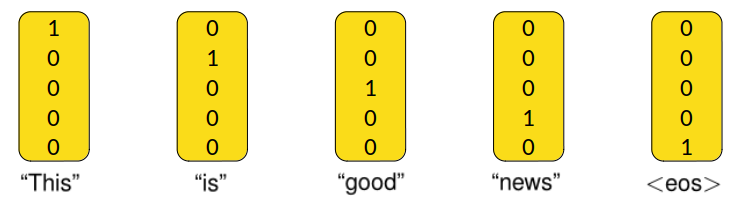
\includegraphics{figure/one_hot_1.png}}
  \end{figure}
    While this is one option to represent words in a network, the standard approach are word embeddings (more on this later).
  \end{itemize}
\end{frame}

\begin{frame} {RNNs - Introduction}
  \begin{itemize}
    \item Our goal is to feed the words to the network sequentially in discrete time-steps.
    \item A regular dense neural network with a single hidden layer only has two sets of weights: 'input-to-hidden' weights $\mathbf{W}$ and 'hidden-to- output' weights $\mathbf{U}$.
  \end{itemize}
  \begin{figure}
      \centering
      \scalebox{0.7}{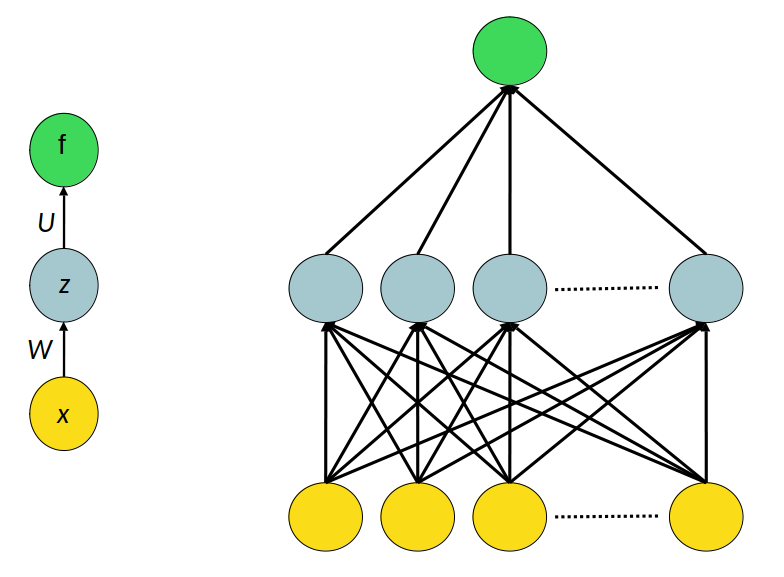
\includegraphics{figure/ffwd1.png}}
  \end{figure}
\end{frame}

\begin{frame} {RNNs - Introduction}
  \begin{itemize}
    \item \small{In order to enable the network to retain information about past inputs, we introduce an \textbf{additional set of weights} $\mathbf{V}$, from the hidden neurons at time-step $t$ to the hidden neurons at time-step $t+1$.
    \item Having this additional set of weights makes the activations of the hidden layer depend on \textbf{both} the current input and the activations for the \textit{previous} input.}
  \end{itemize}
  \begin{figure}
      \centering
      \scalebox{0.80}{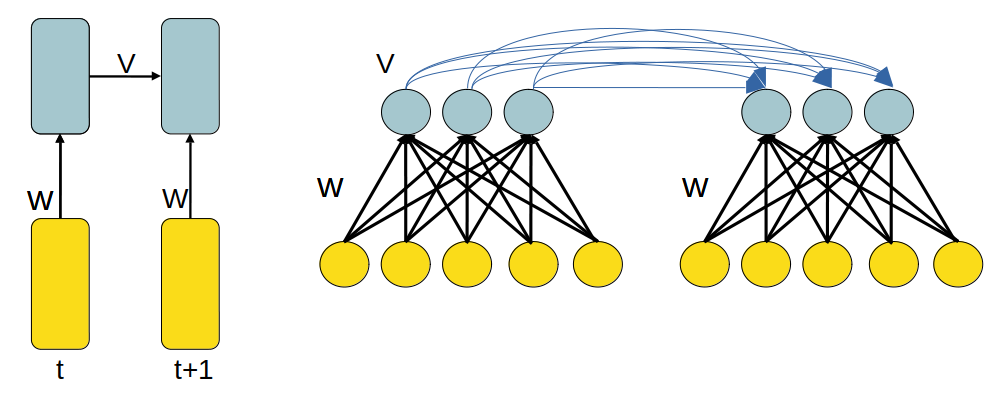
\includegraphics{figure/hidrohid.png}}
      \caption{\footnotesize Input-to-hidden weights $\mathbf{W}$ and \textbf{hidden-to-hidden} weights $\mathbf{V}$. The hidden-to-output weights $\mathbf{U}$ are not shown for better readability.}
  \end{figure}
\end{frame}

\begin{frame} {RNNs - Introduction}
  \begin{itemize}
    \item With this additional set of hidden-to-hidden weights $\mathbf{V}$, the network is now a Recurrent Neural Network (RNN).
    \item In a regular feed-forward network, the activations of the hidden layer are only computed using the input-hidden weights $\mathbf{W}$ (and bias $\mathbf{b}$).
    $$\mathbf{z}= \sigma(\mathbf{W}^\top \xv + \mathbf{b})$$
    \item In an RNN, the activations of the hidden layer (at time-step $t$) are computed using \textit{both} the input-to-hidden weights $W$ and the hidden-to-hidden weights $\mathbf{V}$.
    $$\mathbf{z}^{[t]} = \sigma(\mathbf{\textcolor{red}{\mathbf{V}^\top\mathbf{z}^{[t-1]}}} + \mathbf{W}^\top \mathbf{x}^{[t]} + \mathbf{b})$$
    \item The vector $\mathbf{z}^{[t]}$ represents the short-term memory of the RNN because it is a function of the current input $\mathbf{x}^{[t]}$ and the activations $\mathbf{z}^{[t-1]}$ of the previous time-step.
    \item Therefore, by recurrence, it contains a "summary" of \textit{all} previous inputs. 
  \end{itemize}
\end{frame}

\section{Examples}


\begin{frame} {Application example - Sentiment Analysis}
  \begin{itemize}
    \item At $t = 0$, we feed the word "This" to the network and obtain $\mathbf{z}^{[0]}$.
    \item $\mathbf{z}^{[0]} = \sigma(\mathbf{W}^\top \mathbf{x}^{[0]} + \mathbf{b})$
  \end{itemize}
  \begin{figure}
      \centering
      \scalebox{0.55}{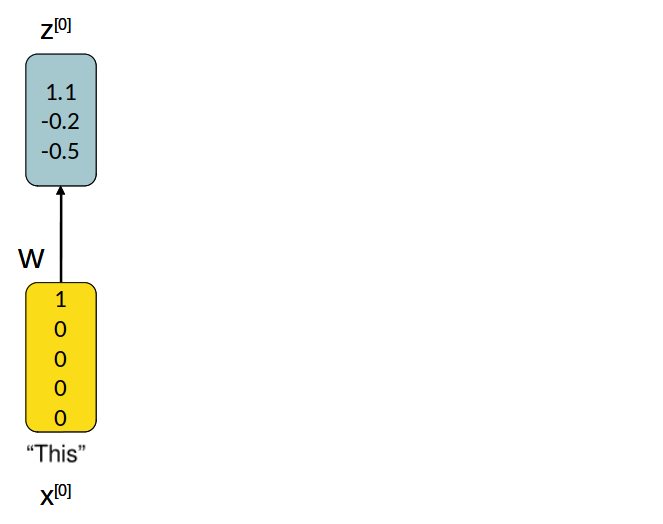
\includegraphics{figure/rnn_sample_z0.png}}
  \end{figure}
  Because this is the very first input, there is no past state (or, equivalently, the state is initialized to 0).
\end{frame}

\begin{frame} {Application example - Sentiment Analysis}
  \begin{itemize}
    \item At $t = 1$, we feed the second word to the network to obtain $\mathbf{z}^{[1]}$.
    \item $\mathbf{z}^{[1]} = \sigma(\mathbf{V}^\top\textcolor{red}{\mathbf{z}^{[0]}} + \mathbf{W}^\top \xv^{[1]} + \mathbf{b})$
  \end{itemize}
  \begin{figure}
      \centering
      \scalebox{0.55}{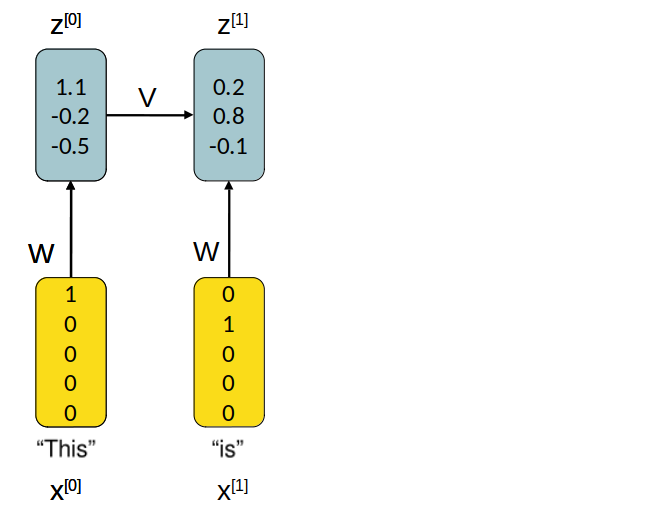
\includegraphics{figure/rnn_sample_z1.png}}
  \end{figure}
\end{frame}

\begin{frame} {Application example - Sentiment Analysis}
  \begin{itemize}
    \item At $t = 2$, we feed the next word in the sentence.
    \item $\mathbf{z}^{[2]} = \sigma(\mathbf{V}^\top\textcolor{red}{\mathbf{z}^{[1]}} + \mathbf{W}^\top \xv^{[2]} + \mathbf{b})$
  \end{itemize}
  \begin{figure}
      \centering
      \scalebox{0.55}{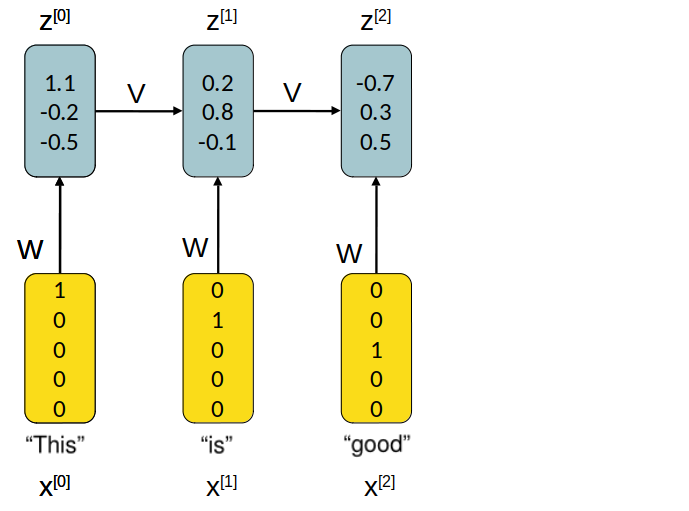
\includegraphics{figure/rnn_sample_z2.png}}
  \end{figure}
\end{frame}

\begin{frame} {Application example - Sentiment Analysis}
  \begin{itemize}
    \item At $t = 3$, we feed the next word ("news") in the sentence.
    \item $\mathbf{z}^{[3]} = \sigma(\mathbf{V}^\top\textcolor{red}{\mathbf{z}^{[2]}} + \mathbf{W}^\top \xv^{[3]} + \mathbf{b})$
  \end{itemize}
  \begin{figure}
      \centering
      \scalebox{0.65}{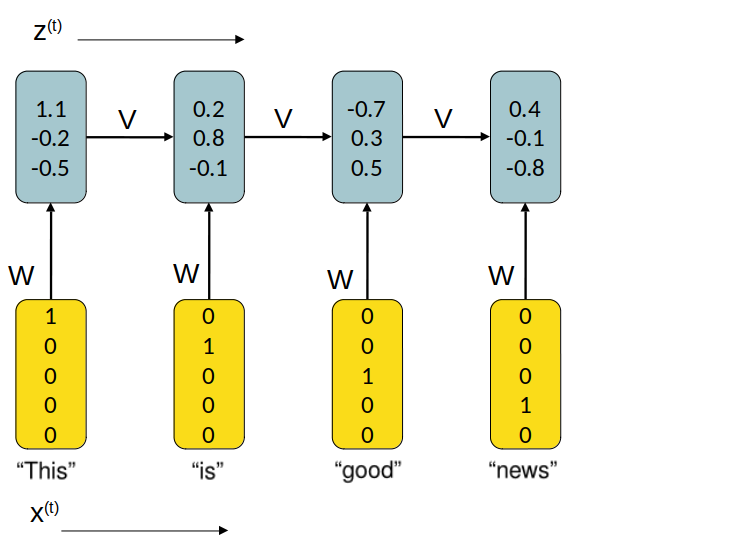
\includegraphics{figure/rnn_sample_z3.png}}
  \end{figure}
\end{frame}

\begin{frame} {Application example - Sentiment Analysis}
  \begin{itemize}
    \item Once the entire input sequence has been processed, the prediction of the network can be generated by feeding the activations of the final time-step to the output neuron(s).
    \item $f = \sigma (\mathbf{U}^\top \mathbf{z}^{[4]} + {c})$, where $c$ is the bias of the output neuron.
  \end{itemize}
  \begin{figure}
      \centering
      \scalebox{0.65}{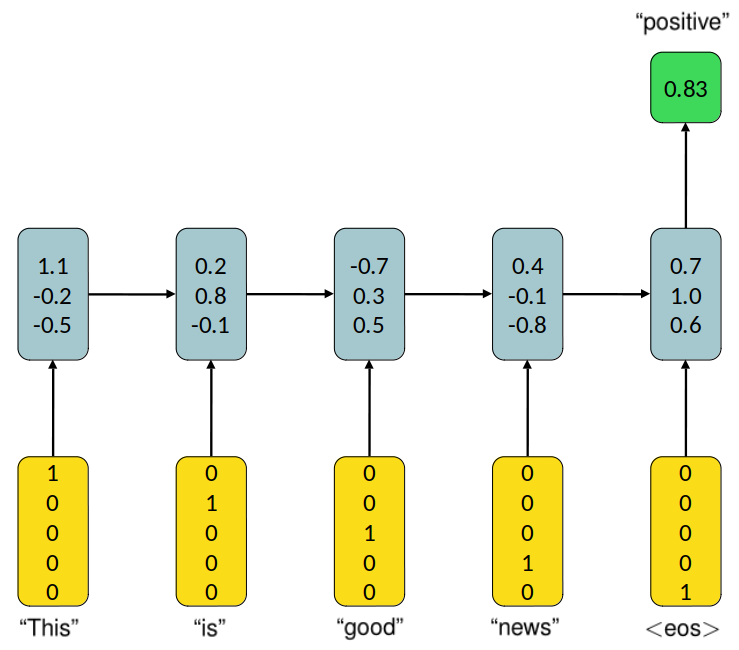
\includegraphics{figure/rnn_sample_z5.png}}
  \end{figure}
\end{frame}

\begin{frame} {Parameter Sharing}
  \begin{itemize}
    \item This way, the network can process the sentence one word at a time and the length of the network can vary based on the length of the sequence.
    \item It is important to note that no matter how long the input sequence is, the matrices $\mathbf{W}$ and $\mathbf{V}$ are the same in every time-step. This is another example of \textbf{parameter sharing}.
    \item Therefore, the number of weights in the network is independent of the length of the input sequence.
  \end{itemize}
\end{frame}

%\begin{frame} {Sequence Modeling - Design Criteria}
%
%To model sequences we need to:
%
%
%  \begin{itemize}
%    \item Handle variable-length sequence,
%    \item Track long-term dependencies,
%    \item Maintain information about order,
%    \item Share parameter across the sequence.
%  \end{itemize}
%
%  \begin{figure}
%      \centering
%      \scalebox{0.2}{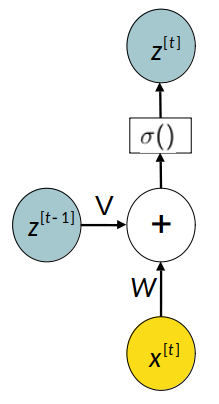
\includegraphics{figure/vanilla_rnn.png}}
%      \caption{\footnotesize {Vanilla RNN}}
%  \end{figure}
%
%\end{frame}

\begin{frame} {RNNs - Use Case specific architectures}

  \small{RNNs are very versatile. They can be applied to a wide range of tasks.
  
  \begin{figure}
      \centering
      \scalebox{0.9}{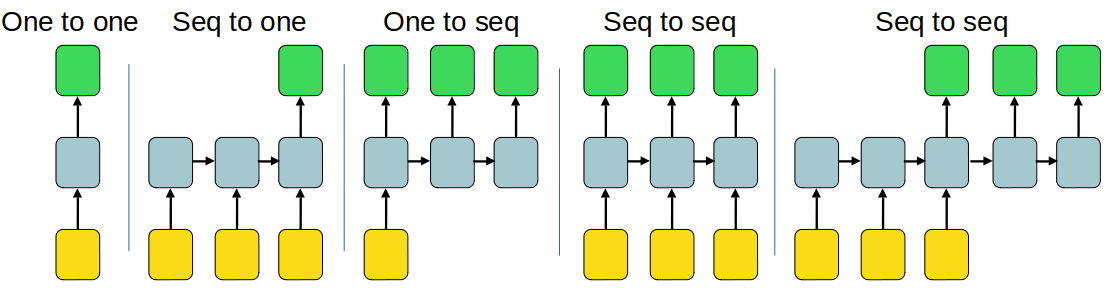
\includegraphics{figure/one_to_one.png}}
      \caption{\footnotesize {RNNs can be used in tasks that involve multiple inputs and/or multiple outputs. }}
  \end{figure}
  Examples:}
  \begin{itemize}
    \item \small{Sequence-to-One: Sentiment analysis, document classification.
    \item One-to-Sequence: Image captioning.
    \item Sequence-to-Sequence: Language modelling, machine translation, time-series prediction.}
  \end{itemize}
\end{frame}


%%%%%%%%%%%%%%%%%%%%%%%%%%%%%%%%%%%%%%%%%%%%%%%%%%%%%%%%%%%%%%%%%%
%%%%%%%%%%%%%%%%%%%%%%%%%%%%%%%%%%%%%%%%%%%%%%%%%%%%%%%%%%%%%%%%%%

\section{Computational Graph}

\frame{
\frametitle{RNNs - Computational Graph}
  \center
  \begin{figure}%
    \only<1>{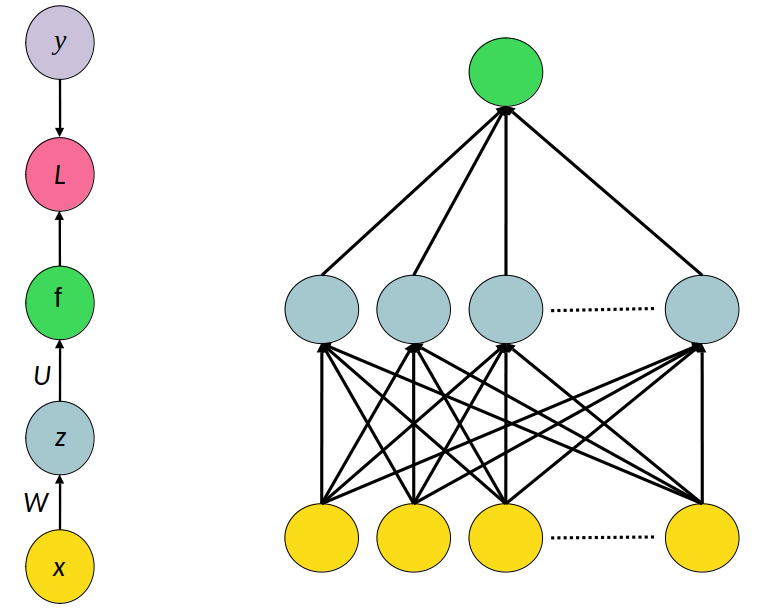
\includegraphics[width=7cm]{figure/nonrecurrent.png}}%
%   \only<2-3>{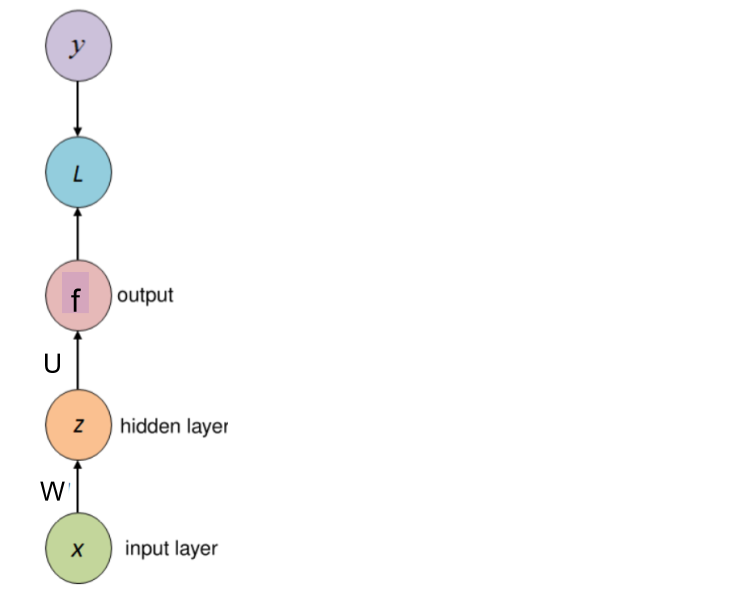
\includegraphics[width=7cm]{plots/rnn_comp2.png}}%
    \only<2>{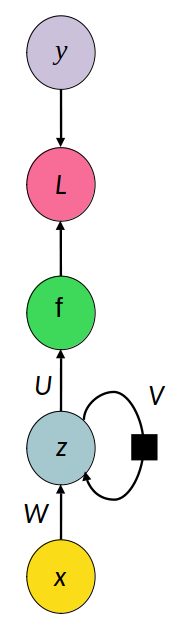
\includegraphics[width=1.5cm]{figure/recurrent_single.png}}%
    \only<3-4>{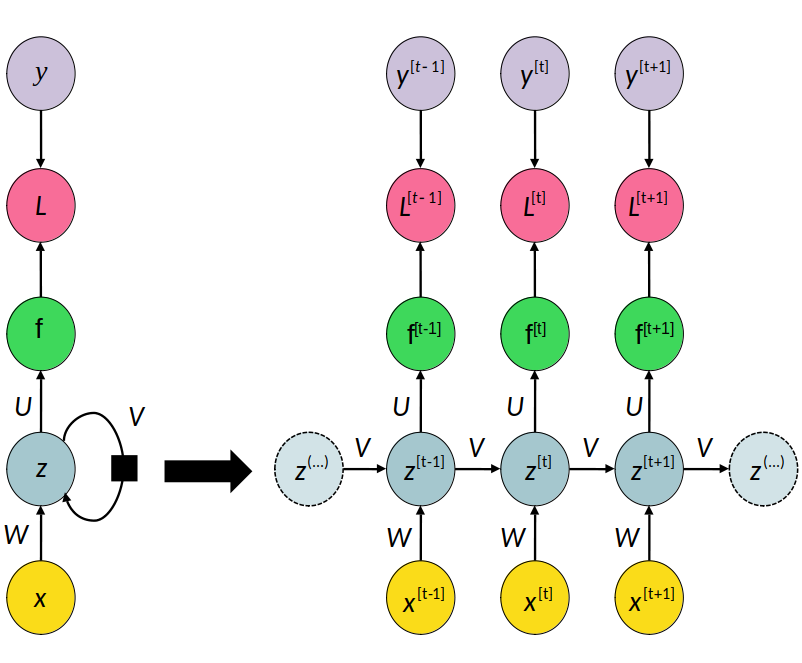
\includegraphics[width=7cm]{figure/recurrent_unfolded.png}}%
    \only<5>{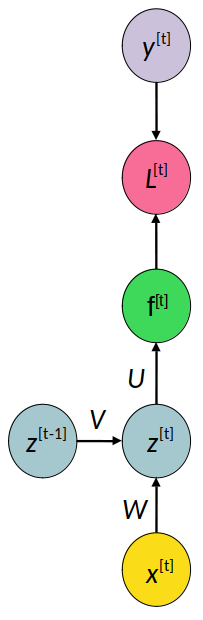
\includegraphics[width=1.5cm]{figure/rnn_zt_figure.png}}%
  \end{figure}%
  \vspace{-0.2cm}
  \begin{itemize}
    \only<1>{\item On the left is an abstract representation of the computational graph for the network on the right. A loss function $L$ measures how far each output
    $f$ is from the corresponding training target $y$. }
    % \only<2-3>{\item In order to derive RNNs we have to extend our notation.}
    % \only<3>{\begin{itemize}
    %   \only<3>{\item So far, we mapped some inputs $x$ to outputs $f$:}
    %   \only<3>{\item[] $f = \tau(c + U^T z) = \tau(c + U^T \sigma(b + W^T x))$}
    %   \only<3>{\item[] ..with $W$ and $U$ being weight matrices.}
    % \end{itemize}}
    \only<2>{\item A helpful way to think of an RNN is as multiple copies of the same network, each passing a message to a successor.}
    \only<2>{\item RNNs are networks with loops, allowing information to persist.}
    \only<3>{\item Things might become more clear if we unfold the architecture.}
    \only<3>{\item We call $\mathbf{z}^{[t]}$ the \textit{state} of the system at time $t$.}
    \only<3>{\item Tthe state contains information about the whole past sequence.}
    \only<4>{\item We went from 
      \begin{eqnarray*} 
        f &=& \tau(c + \mathbf{U}^\top \sigma(\mathbf{b} + \mathbf{W}^\top \mathbf{x})) \text{ for the dense net, to } \\
        f^{[t]} &=& \tau(c + \mathbf{U}^\top \sigma(\mathbf{b} + \mathbf{V}^\top \mathbf{z}^{[t-1]} + \mathbf{W}^\top \xv^{[t]})) \text{ for the RNN. }
      \end{eqnarray*}}
    \only<5>{\item A potential computational graph for time-step $t$ with}
    \only<5>{\item[] $$f^{[t]} = \tau(c + \mathbf{U}^\top \sigma(\mathbf{b} + \mathbf{V}^\top \mathbf{z}^{[t-1]} + \mathbf{W}^\top \xv^{[t]})) $$ }
  \end{itemize}
}


\frame{
\frametitle{Recurrent output-hidden connections}

Recurrent connections do not need to map from hidden to hidden neurons!

\center
\begin{figure}
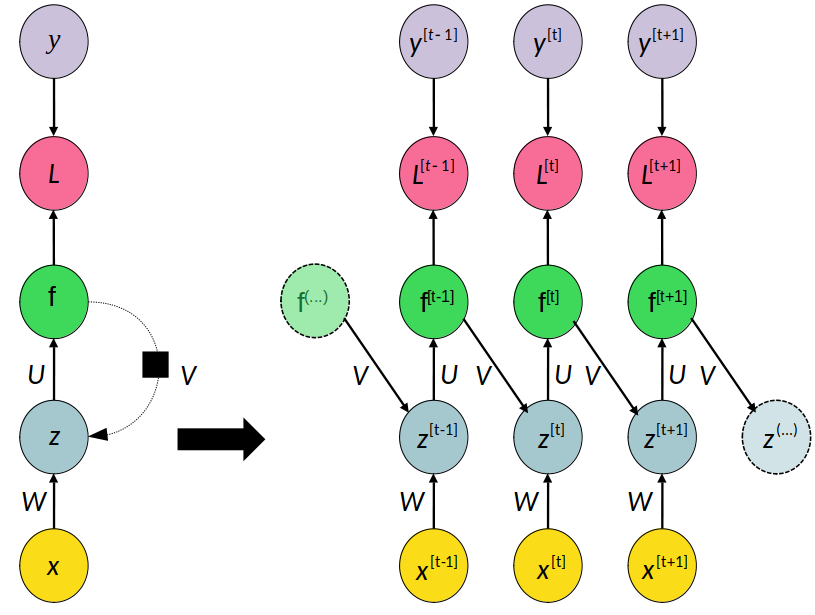
\includegraphics[width=7cm]{figure/recurrent_unfolded_fromoutput.png} 
\end{figure}
 \footnotesize{RNN with feedback connection from the output to the hidden layer. The RNN is only allowed to send $f$ to future time points and, hence, $z^{[t-1]}$ is connected to $z^{[t]}$ only indirectly, via the predictions $f^{[t-1]}$.}

}

\frame{
\frametitle{Seq-to-one mappings}

RNNs do not need to produce an output at each time step. Often only one output is produced after processing the whole sequence. 

\center
\begin{figure}
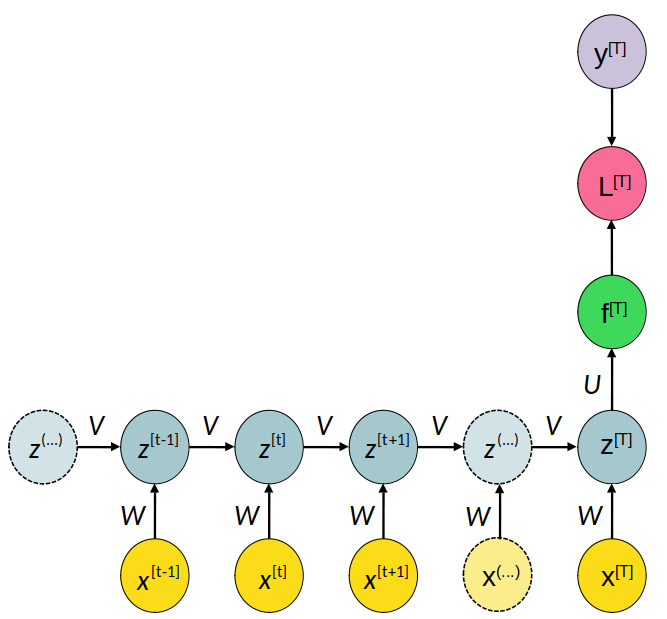
\includegraphics[width=5cm]{figure/rnn_last_output.png} 
     \footnotesize{\\Time-unfolded recurrent neural network with a single output at the end of the sequence. Such a network can be used to summarize a sequence and produce a fixed size representation.}
\end{figure}

}



%%%%%%%%%%%%%%%%%%%%%%%%%%%%%%%%%%%%%%%%%%%%%%%%%%%%%%%%%%%%%%%%%%
%%%%%%%%%%%%%%%%%%%%%%%%%%%%%%%%%%%%%%%%%%%%%%%%%%%%%%%%%%%%%%%%%%
%%%%%%%%%%%%%%%%%%%%%%%%%%%%%%%%%%%%%%%%%%%%%%%%%%%%%%%%%%%%%%%%%%
%%%%%%%%%%%%%%%%%%          REFERENCES          %%%%%%%%%%%%%%%%%%
%%%%%%%%%%%%%%%%%%%%%%%%%%%%%%%%%%%%%%%%%%%%%%%%%%%%%%%%%%%%%%%%%%
\begin{vbframe}
\frametitle{References}
\footnotesize{
\begin{thebibliography}{99}
%%%%%%%%%%%%%%%%%%%%%%%%%%%%%%%%%%
\bibitem[Ian Goodfellow et al., 2016]{1} Ian Goodfellow, Yoshua Bengio and Aaron Courville (2016)
\newblock Deep Learning
\newblock \emph{\url{http://www.deeplearningbook.org/}}
%%%%%%%%%%%%%%%%%%%%%%%%%%%%%%%%%%
\bibitem[Andrej Karpathy., 2015]{1} Andrej Karpathy (2015)
\newblock The Unreasonable Effectiveness of Recurrent Neural Networks
\newblock \emph{\url{http://karpathy.github.io/2015/05/21/rnn-effectiveness/}}
%%%%%%%%%%%%%%%%%%%%%%%%%%%%%%%%%%
\end{thebibliography}
}
\end{vbframe}
%%%%%%%%%%%%%%%%%%%%%%%%%%%%%%%%%%%%%%%%%%%%%%%%%%%%%%%%%%%%%%%%%%
%%%%%%%%%%%%%%%%%%%%%%%%%%%%%%%%%%%%%%%%%%%%%%%%%%%%%%%%%%%%%%%%%%

\endlecture
\end{document}